\chapter{Interfaz web y asistente conversacional}
\label{anexo:interfaz}

La interfaz web \framework\ (aplicación Streamlit) es el punto de acceso
público al framework. Se ha diseñado con dos objetivos: (i) que un
revisor pueda navegar por los resultados del trabajo sin necesidad de
leer código, y (ii) que cualquier cifra citada en la memoria sea
verificable en tiempo real contra los CSV/JSON que produce el pipeline.
Este anexo describe la interfaz vista a vista, explicando qué se ve en
cada pantalla y de dónde salen los datos.

\section*{Arquitectura de la aplicación}
\addcontentsline{toc}{section}{Arquitectura de la aplicación}

La aplicación se implementa como un sitio multipágina de Streamlit
compuesto por tres módulos Python:

\begin{itemize}
  \item \texttt{paso12\_web\_chatbot.py} es el \emph{router}: configura
  la página (título, favicon, layout) y registra dos vistas con
  \texttt{st.navigation}: la \emph{landing} en la ruta raíz \texttt{/} y
  el \emph{framework} en \texttt{/framework}. Ambas vistas se ocultan de
  la navegación lateral automática de Streamlit (\texttt{position="hidden"})
  y se enlazan con botones propios.
  \item \texttt{paso12\_landing.py} contiene la vista de portada
  minimalista.
  \item \texttt{paso12\_dashboard.py} contiene la vista de trabajo con
  siete capítulos.
\end{itemize}

Los datos que consumen ambas vistas se leen desde
\texttt{paso12\_datos.py}, que se encarga de agregar métricas y publicar
funciones puras (\texttt{metricas()}, \texttt{resumen\_firma()},
\texttt{tabla()}, \texttt{dec()}) usadas por toda la interfaz. Esta
separación estricta entre presentación y datos garantiza que cualquier
cifra mostrada sea trazable a una fila concreta de los CSV/JSON. La
figura~\ref{fig:arquitectura} resume la arquitectura completa de la
interfaz.

\begin{figure}[H]
  \centering
  \begin{tikzpicture}[node distance=0.5cm and 0.9cm]
    % Datos
    \node[entrada, minimum width=2.6cm] (csv) {CSV / JSON\\del pipeline};
    % Capa de datos
    \node[paso, right=1.2cm of csv] (datos) {\texttt{paso12\_datos.py}\\metricas() · tabla()};
    \node[paso, below=0.35cm of datos] (ctx)   {\texttt{contexto\_tfm.py}\\prompt sistema};
    % Router
    \node[paso, right=1.2cm of datos] (router) {\texttt{paso12\_web\_chatbot.py}\\router \texttt{st.navigation}};
    % Vistas
    \node[salida, right=1.2cm of router, yshift=0.7cm] (landing) {Portada\\\texttt{/}};
    \node[salida, right=1.2cm of router, yshift=-0.7cm] (dash)    {Framework\\\texttt{/framework}};
    % Groq
    \node[entrada, below=0.7cm of ctx] (groq) {API Groq\\Llama 3.3-70b};

    % Flechas
    \draw[flecha] (csv) -- (datos);
    \draw[flecha] (csv.south) |- (ctx.west);
    \draw[flecha] (datos) -- (router);
    \draw[flecha] (ctx.east) -| ($(router.south)+(0,-0.3)$) -- (router.south);
    \draw[flecha] (router.east) -- (landing.west);
    \draw[flecha] (router.east) -- (dash.west);
    \draw[flecha, dashed] (groq) -- (ctx);
  \end{tikzpicture}
  \caption{Arquitectura de la interfaz web. Los CSV/JSON del pipeline
  se leen desde \texttt{paso12\_datos.py} (datos) y
  \texttt{contexto\_tfm.py} (prompt del asistente). El router de
  \texttt{paso12\_web\_chatbot.py} expone dos vistas: la portada
  (\texttt{/}) y el dashboard del framework (\texttt{/framework}). La
  línea discontinua indica la dependencia externa opcional (API de
  Groq) del asistente conversacional.}
  \label{fig:arquitectura}
\end{figure}

Para ejecutar la aplicación localmente:

\begin{lstlisting}[style=bash, caption={Ejecución de la interfaz.}]
streamlit run agentes/paso12_web_chatbot.py
\end{lstlisting}

La aplicación se abre por defecto en \url{http://localhost:8501}. El
asistente conversacional requiere una clave API de Groq configurada en
el fichero \texttt{.env} de la raíz (\texttt{GROQ\_API\_KEY=gsk\_\dots});
sin esta clave el resto de la interfaz funciona con normalidad y sólo se
deshabilita el chat.

\section*{Vista 1: Portada}
\addcontentsline{toc}{section}{Vista 1: Portada}

La portada (figura~\ref{fig:if_landing}) presenta el nombre del
framework en tipografía monoespaciada con un punto verde de acento
(\emph{data.lung}) y una tagline breve. Sobre el nombre corre en
segundo plano una animación estilo terminal con las trazas reales del
pipeline (descargas, curación LLM, análisis diferencial, folds LODO),
que enfatiza que el trabajo es reproducible. El botón central
\emph{Comenzar} redirige a la vista de framework. A la derecha se
incluye una decoración SVG con iconografía biológica (pulmones, doble
hélice, bases nitrogenadas y adenina) inyectada como \texttt{data:URI}
para sortear el saneado HTML de Streamlit.

\begin{figure}[H]
  \centering
  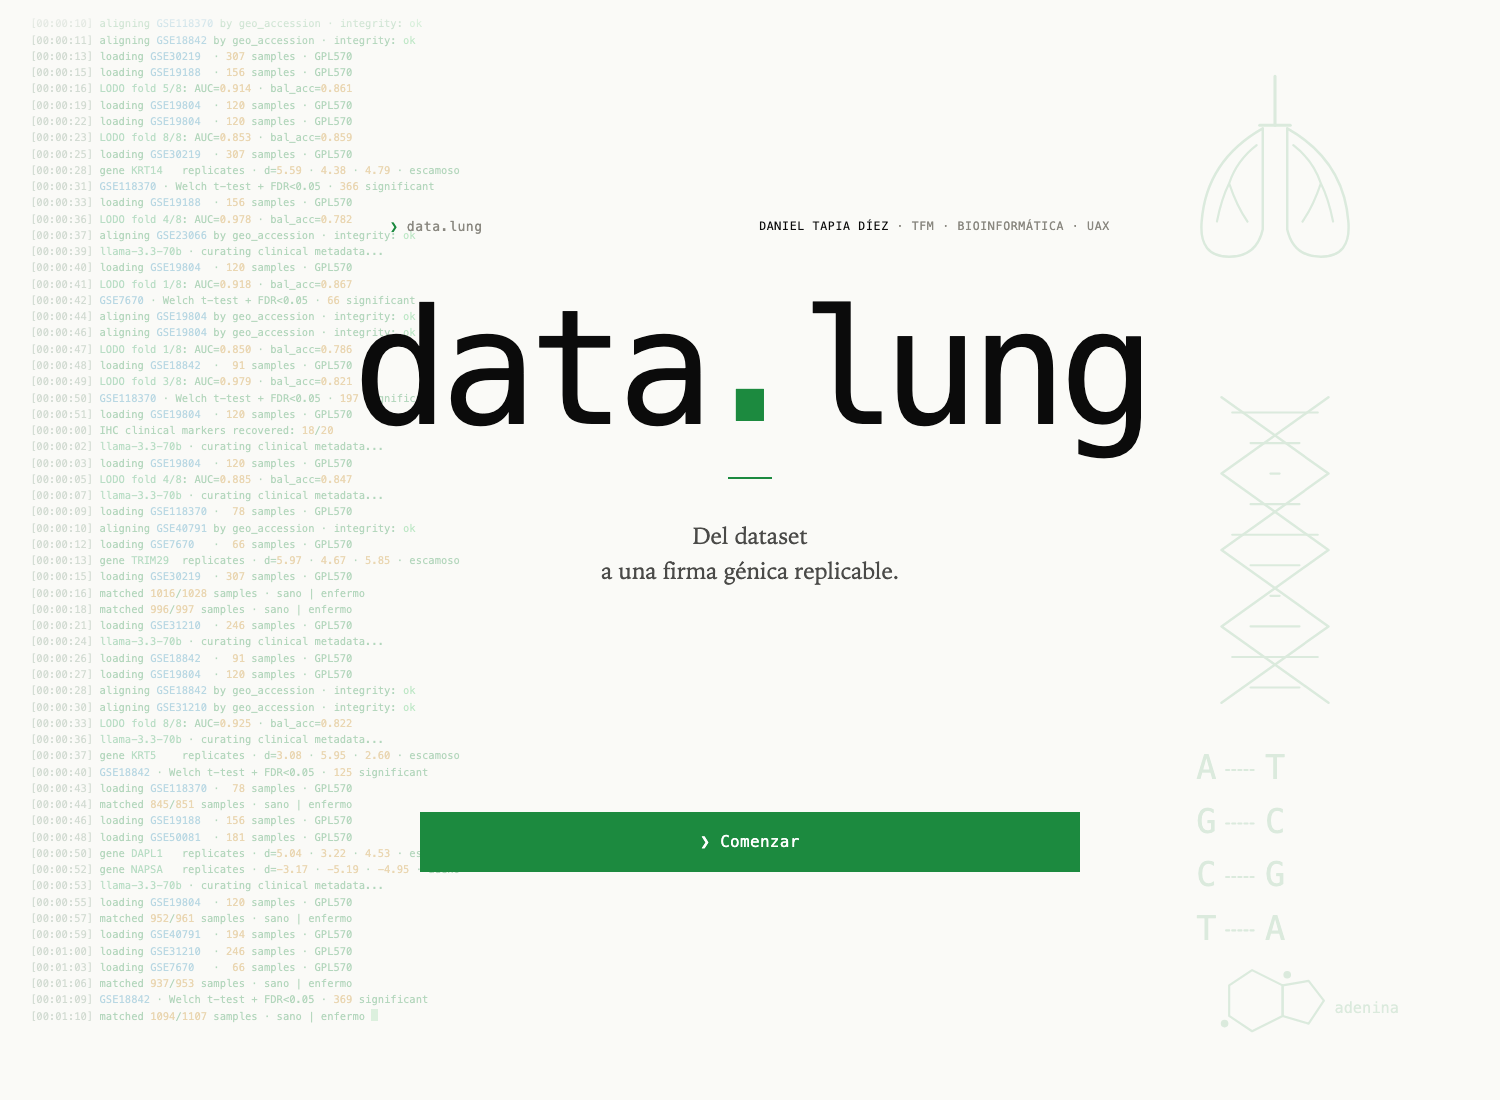
\includegraphics[width=0.9\linewidth]{figuras/interfaz/01_landing.png}
  \caption{Portada de la interfaz \framework. Fondo con terminal animada
  reproduciendo trazas reales del pipeline, tipografía mono con acento
  verde y CTA \emph{Comenzar}.}
  \label{fig:if_landing}
\end{figure}

\section*{Vista 2: Framework - capítulo \emph{Inicio}}
\addcontentsline{toc}{section}{Vista 2: Framework - capítulo Inicio}

Al entrar en \texttt{/framework} se aterriza en el capítulo
\emph{Inicio} (figura~\ref{fig:if_inicio}), que muestra:

\begin{itemize}
  \item Una marca superior en tipografía monoespaciada
  ``\texttt{> data.lung \textperiodcentered\ framework}''.
  \item El kicker \emph{Trabajo de Fin de Máster · Bioinformática · UAX}.
  \item El título completo del trabajo.
  \item Una entradilla en tipografía serif que resume el framework y
  distingue explícitamente las dos tareas (tumor \emph{vs.} sano y
  subtipo histológico), citando la AUC LODO de la primera.
  \item Un \emph{hero} de cinco tarjetas con las cifras principales,
  con acento verde y numeración animada (\emph{count-up}) al cargar.
\end{itemize}

Las cifras del hero se leen dinámicamente: \texttt{n\_cohortes}
(11) y \texttt{n\_muestras\_curadas} (1157) desde
\texttt{AUDITORIA\_COHORTES.csv}; \texttt{n\_genes\_validados} (1174) y
\texttt{panel\_minimo} (20) desde \texttt{FIRMA\_VALIDADA\_RESUMEN.json};
y AUC media LODO (0,925) desde \texttt{LODO\_HONESTO\_RESULTADOS.csv}.

\begin{figure}[H]
  \centering
  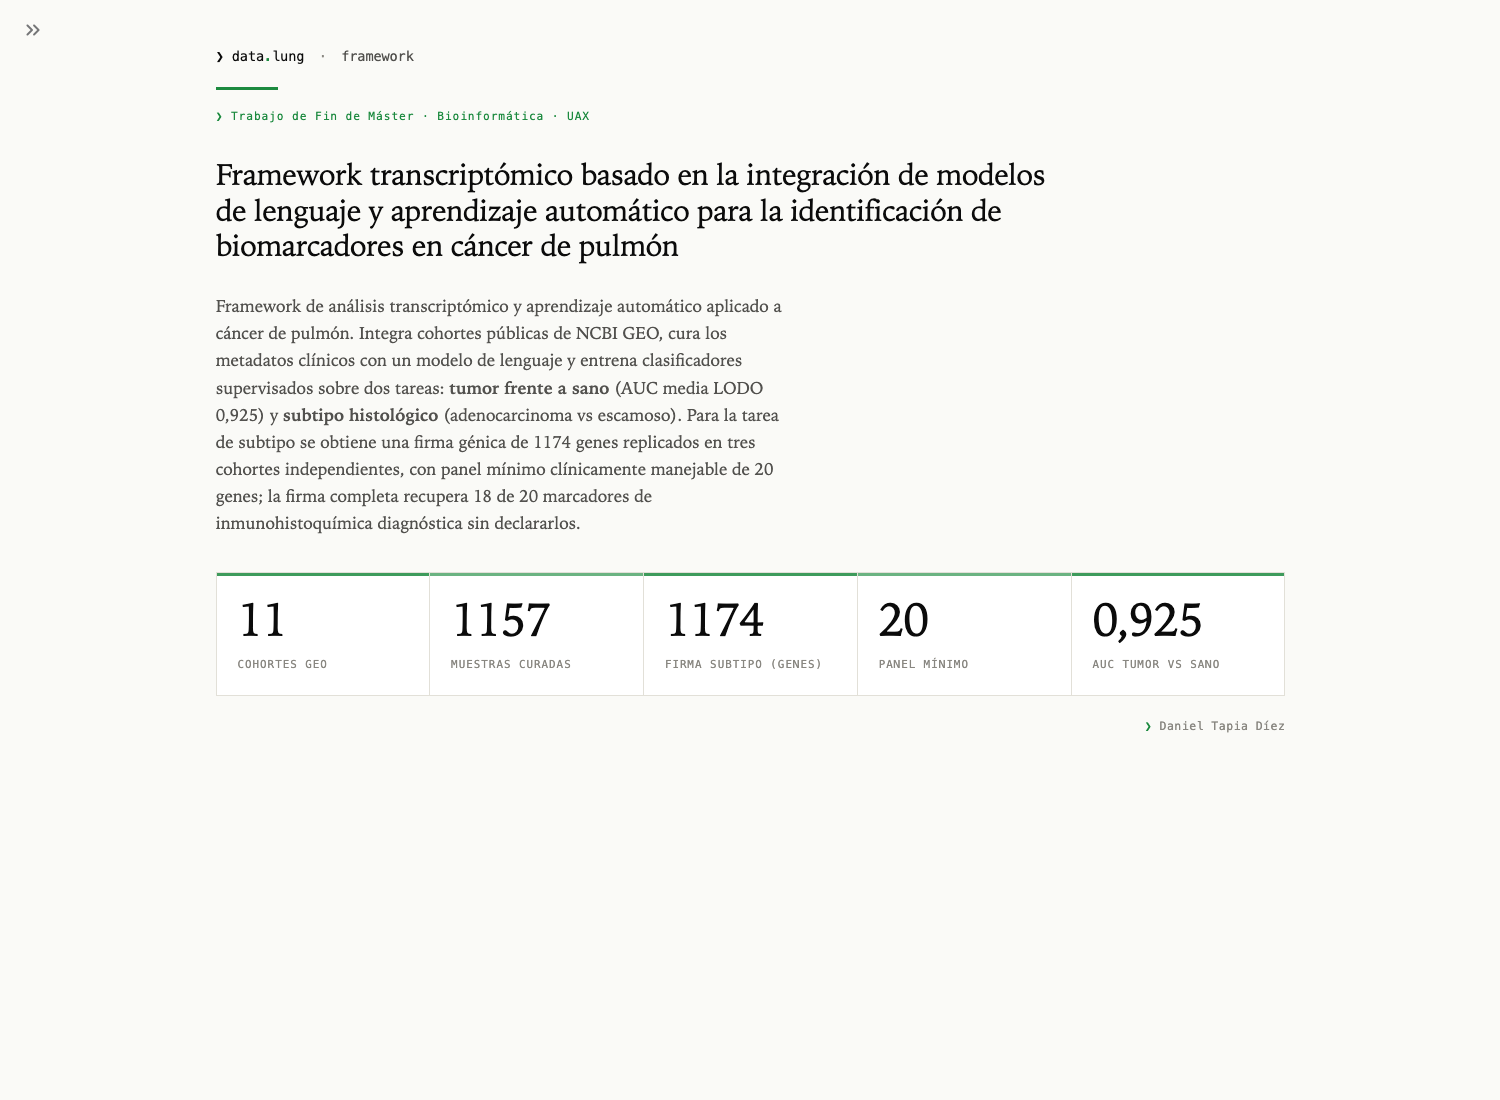
\includegraphics[width=0.9\linewidth]{figuras/interfaz/02_inicio.png}
  \caption{Capítulo \emph{Inicio} del framework. Título, entradilla y
  hero de cinco cifras con acento verde.}
  \label{fig:if_inicio}
\end{figure}

\section*{Vista 3: Asistente conversacional}
\addcontentsline{toc}{section}{Vista 3: Asistente conversacional}

El capítulo \emph{Asistente} (figura~\ref{fig:if_asistente}) integra un
chat con Llama~3.3-70b servido vía Groq. La interfaz consta de:

\begin{itemize}
  \item Una cabecera con avatar circular (icono ADN) y estado en línea.
  \item Un aviso legal breve indicando que el asistente responde
  únicamente con lo que figura en los resultados del trabajo y que no
  proporciona consejo médico ni diagnóstico.
  \item Cuando no hay conversación en curso, seis sugerencias en tres
  columnas (¿De qué trata el proyecto?; ¿Qué biomarcadores identifica?;
  ¿Cuál es el rendimiento del clasificador?; explica los ejes biológicos;
  ¿Cuántos marcadores IHC recupera?; ¿Qué genes forman el panel mínimo?).
  \item Un campo de entrada anclado a la parte inferior del viewport
  (\texttt{st.chat\_input}) con un botón de envío circular verde.
  \item Cuando hay mensajes, cada burbuja lleva un acento vertical
  lateral: verde para el usuario, gris para el asistente, con fondos
  ligeramente tintados. El fondo del asistente está teñido de gris muy
  claro y el del usuario con un verde al 7\,\% de opacidad para
  distinguir visualmente autor sin recurrir al layout iMessage
  (avatares a lados opuestos), que en Streamlit resulta frágil.
\end{itemize}

El asistente se alimenta de un \emph{prompt sistema} construido por
\texttt{contexto\_tfm.py}, cuyo contenido se lee dinámicamente de los
CSV/JSON en cada ejecución (véase anexo~\ref{anexo:prompts}). Las
reglas del prompt le impiden inventar cifras, citar biomarcadores que no
estén en la firma o dar consejo médico. La historia se acota a los
últimos ocho mensajes (cuatro turnos usuario/asistente) para no disparar
el consumo del rate limit de Groq.

\begin{figure}[H]
  \centering
  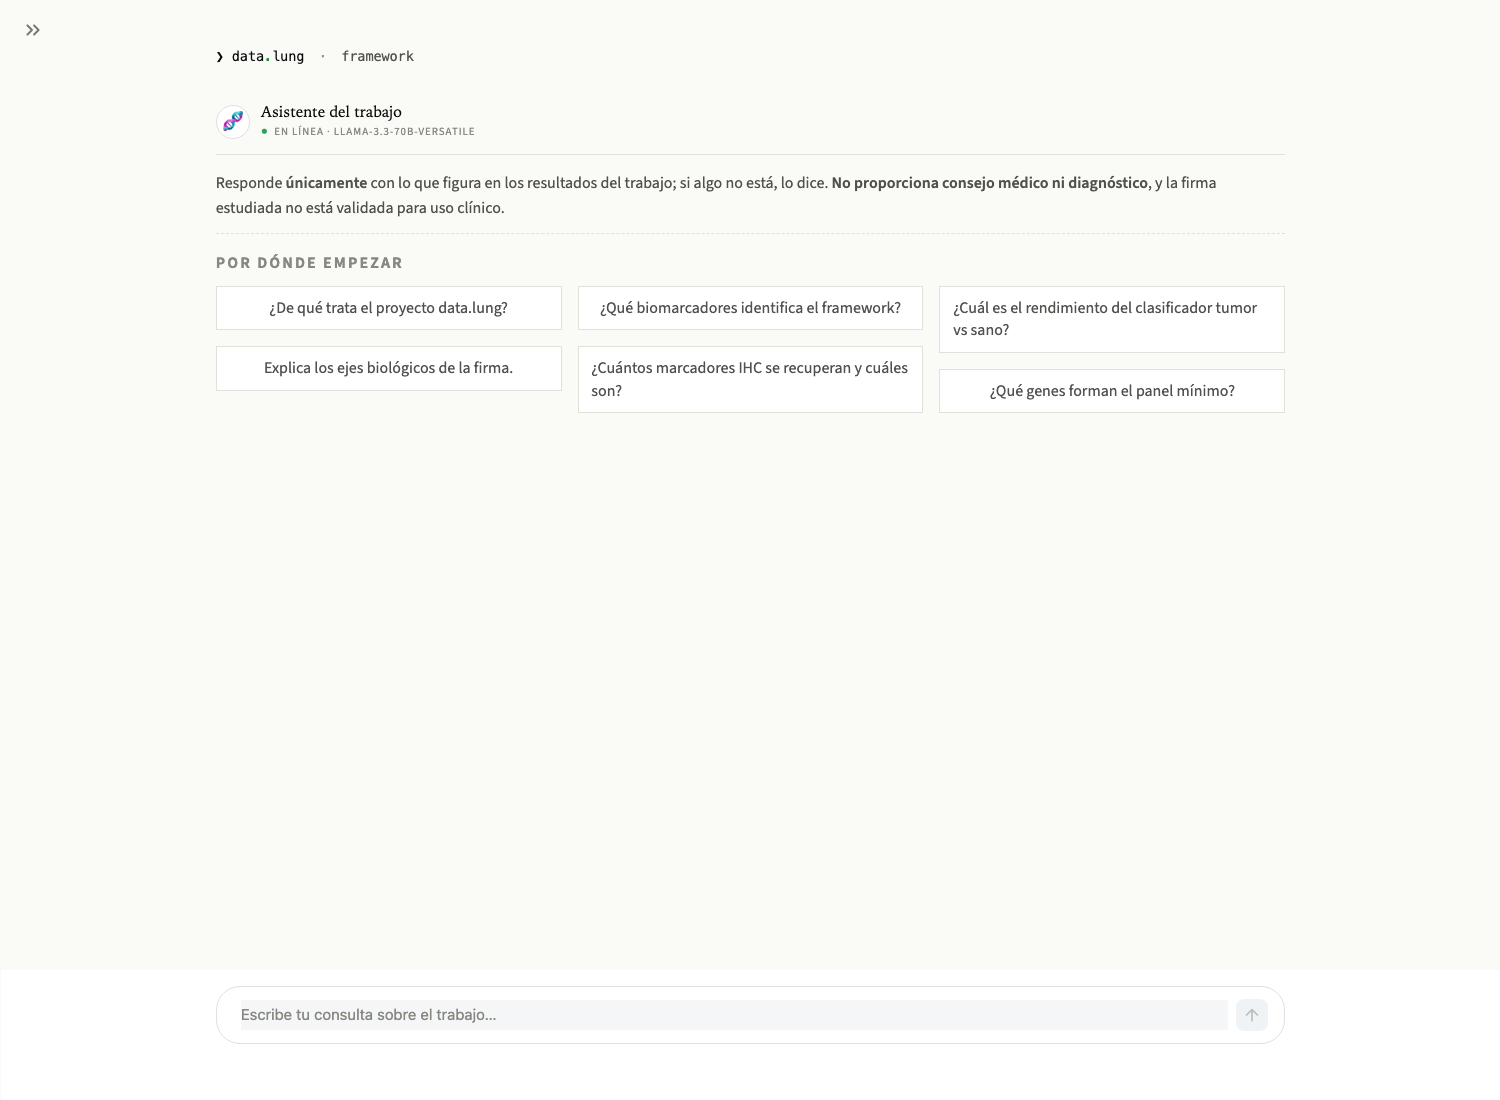
\includegraphics[width=0.9\linewidth]{figuras/interfaz/03_asistente.png}
  \caption{Capítulo \emph{Asistente}. Cabecera con avatar y estado en
  línea, sugerencias iniciales de conversación y input anclado abajo.}
  \label{fig:if_asistente}
\end{figure}

\section*{Vista 4: Introducción y objetivos}
\addcontentsline{toc}{section}{Vista 4: Introducción y objetivos}

Este capítulo (figura~\ref{fig:if_intro}) reproduce en formato web el
contenido de la introducción, los objetivos y la sección
\emph{Datos} del trabajo. Concretamente incluye:

\begin{itemize}
  \item \emph{Sección I}: Contexto y motivación clínica de la elección
  del cáncer de pulmón.
  \item \emph{Sección II}: Objetivo general del framework.
  \item \emph{Sección III}: Lista numerada de objetivos específicos.
  \item \emph{Sección IV}: Tabla dinámica \texttt{AUDITORIA\_COHORTES.csv}
  con las cohortes evaluables, sus tamaños por grupo, la tasa de
  éxito de la curación LLM (representada como barra de progreso) y un
  \emph{caption} que aclara cuántas cohortes cumplen los criterios de
  inclusión y por qué las excluidas quedan fuera.
\end{itemize}

Todas las cifras del caption se computan al vuelo desde el CSV, así que
un cambio en la auditoría se refleja de inmediato en la interfaz.

\begin{figure}[H]
  \centering
  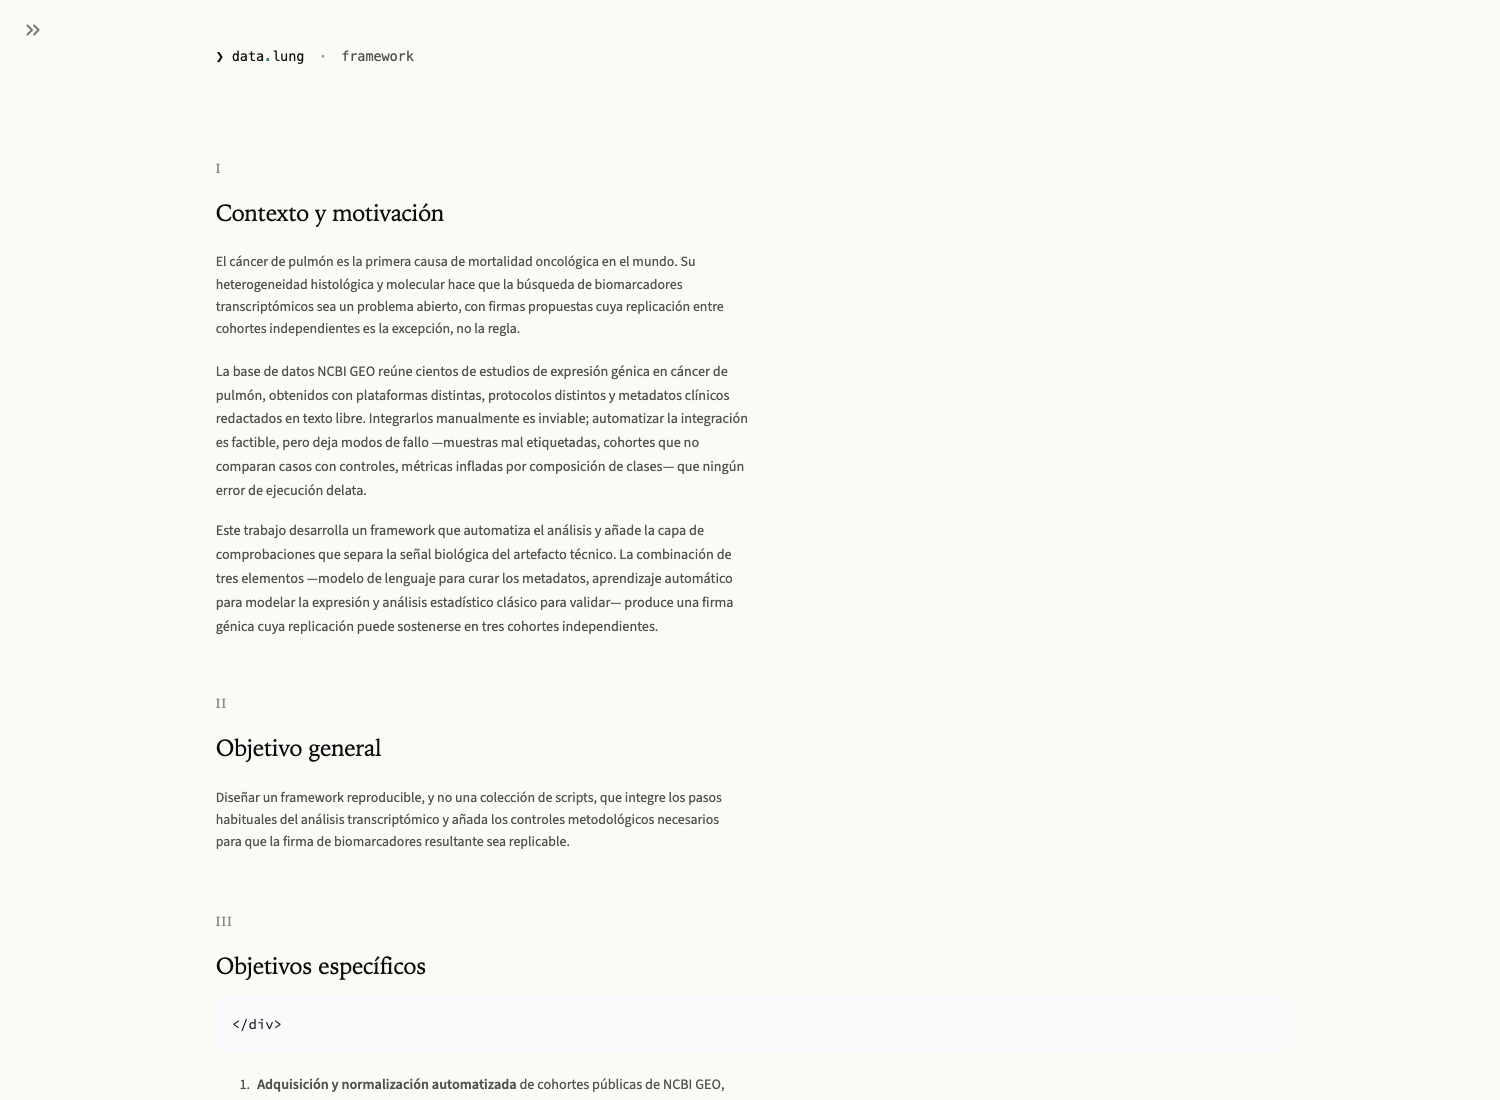
\includegraphics[width=0.9\linewidth]{figuras/interfaz/04_introduccion.png}
  \caption{Capítulo \emph{Introducción y objetivos}. Se aprecia la tabla
  de cohortes con la barra de progreso de curación LLM y el caption
  dinámico.}
  \label{fig:if_intro}
\end{figure}

\section*{Vista 5: Metodología}
\addcontentsline{toc}{section}{Vista 5: Metodología}

El capítulo \emph{Metodología} (figura~\ref{fig:if_metodo}) describe el
pipeline con cinco secciones:

\begin{enumerate}
  \item \emph{Pipeline}: lista numerada de los ocho pasos secuenciales
  del análisis, desde la descarga GEO hasta el determinismo por
  \texttt{random\_state} fijo.
  \item \emph{Curación clínica con modelo de lenguaje}: explica la
  delegación de la traducción de metadatos a Llama~3.3-70b.
  \item \emph{Sobre el efecto lote}: aclara que el framework no aplica
  corrección conjunta de lote porque LODO precisamente lo mide.
  \item \emph{Reproducir los resultados}: bloque con los comandos
  concretos para regenerar la totalidad del árbol de artefactos desde
  la raíz del proyecto.
\end{enumerate}

Este capítulo actúa como \emph{colofón} operativo del trabajo: pega los
comandos que un revisor puede ejecutar para verificar el pipeline sin
salir de la interfaz.

\begin{figure}[H]
  \centering
  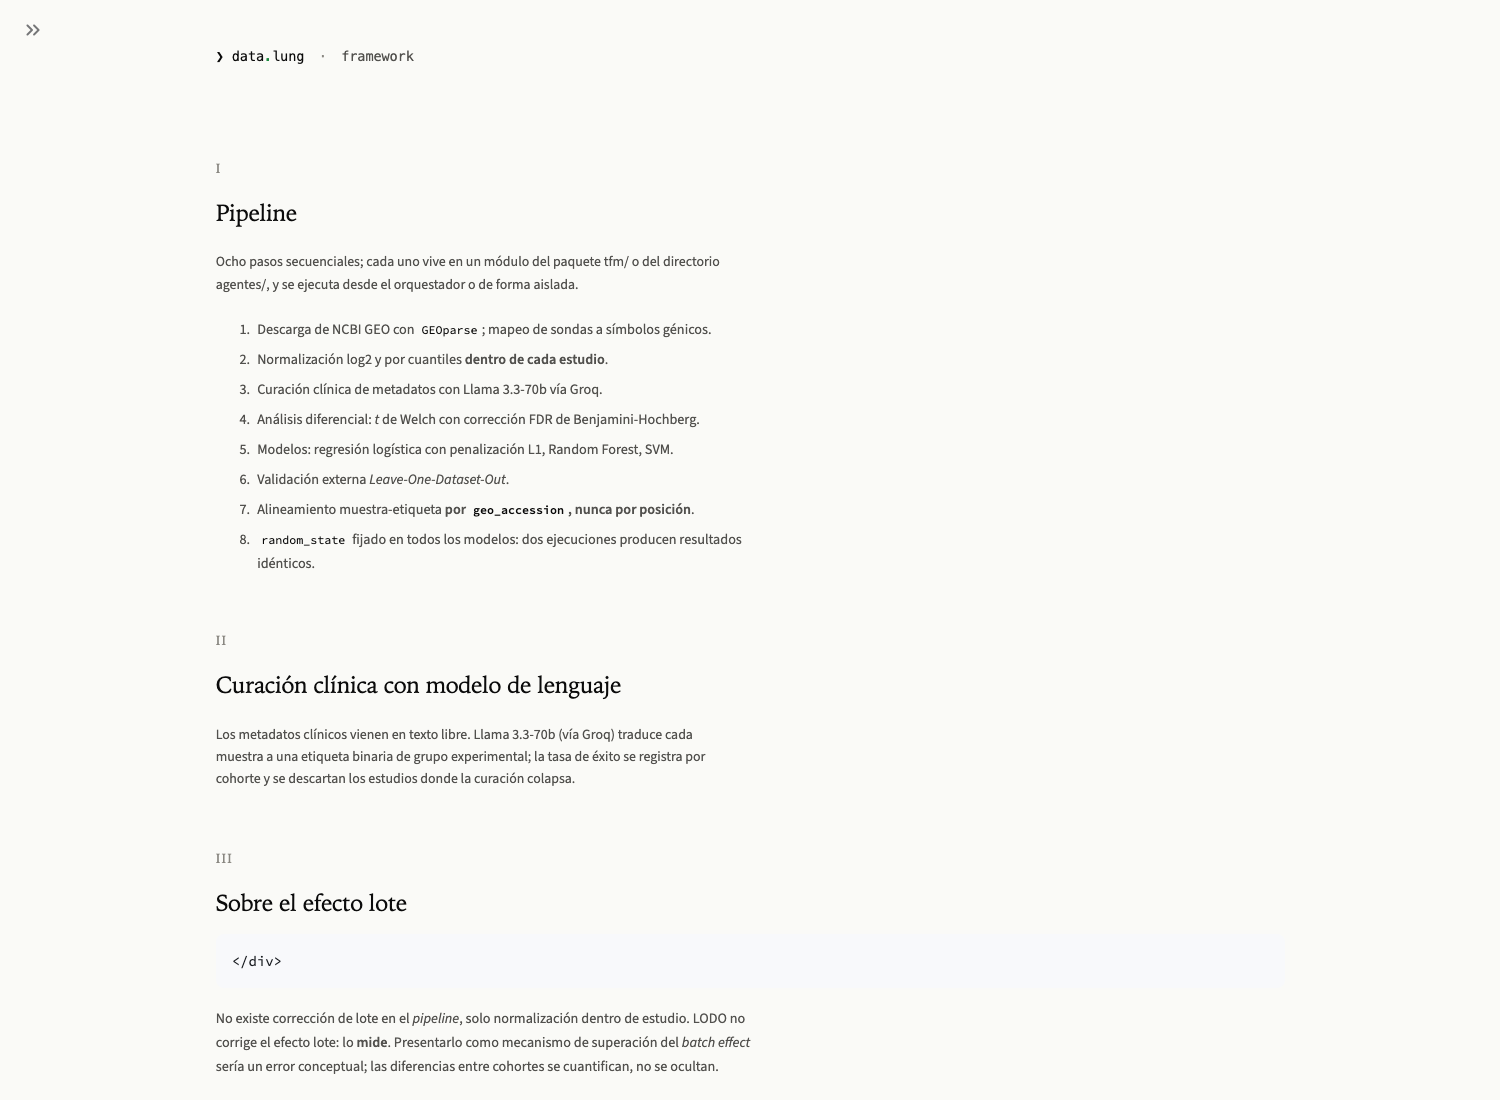
\includegraphics[width=0.9\linewidth]{figuras/interfaz/05_metodologia.png}
  \caption{Capítulo \emph{Metodología}. Bloques numerados con las fases
  del pipeline y comandos de reproducibilidad.}
  \label{fig:if_metodo}
\end{figure}

\section*{Vista 6: Resultados}
\addcontentsline{toc}{section}{Vista 6: Resultados}

El capítulo \emph{Resultados} (figura~\ref{fig:if_res}) es el más denso.
Contiene:

\begin{itemize}
  \item Una cabecera con cuatro tarjetas de cifras principales
  (\emph{genes validados}, \emph{panel mínimo}, \emph{AUC subtipo},
  \emph{marcadores IHC recuperados}) con acento vertical de color.
  \item \emph{Sección I -- Firma génica validada}: describe el resultado
  principal e incluye el \textbf{buscador de gen}. El usuario introduce
  un símbolo génico (\texttt{DSG3}, \texttt{KRT5}, \texttt{NAPSA},
  \texttt{NKX2-1}, \texttt{TP63}, \texttt{MUC1}, \dots) y la interfaz
  responde consultando \texttt{FIRMA\_VALIDADA\_COMPLETA.csv} y
  \texttt{FIRMA\_VALIDADA\_TOP60.csv} en tiempo real: si el gen forma
  parte de la firma, muestra su rango, dirección, $d$ de Cohen en cada
  cohorte y si está en el panel mínimo o coincide con un marcador IHC.
  Bajo el buscador hay un desplegable con la tabla completa del top 60.
  \item \emph{Sección II -- Subtipo histológico}: interpretación
  biológica del panel escamoso vs adenocarcinoma, con las listas
  completas de marcadores IHC recuperados por linaje.
  \item \emph{Sección III -- Tumor vs sano}: métricas medias LODO y
  desplegable con la tabla completa por cohorte.
  \item \emph{Sección IV -- Interpretación biológica}: descripción de
  los dos ejes reales de la firma (pérdida alvéolo-capilar y
  proliferación) con las cifras de correlación leídas del CSV.
  \item \emph{Sección V -- Figuras}: cuatro figuras a ancho completo,
  cada una con descripción de qué muestra y bloque interpretativo con
  borde verde citando la cifra concreta.
\end{itemize}

El buscador de gen es el elemento más útil desde el punto de vista de
auditoría: cualquier revisor puede introducir un símbolo génico y
verificar si aparece en la firma y con qué valores, sin necesidad de
abrir el CSV manualmente.

\begin{figure}[H]
  \centering
  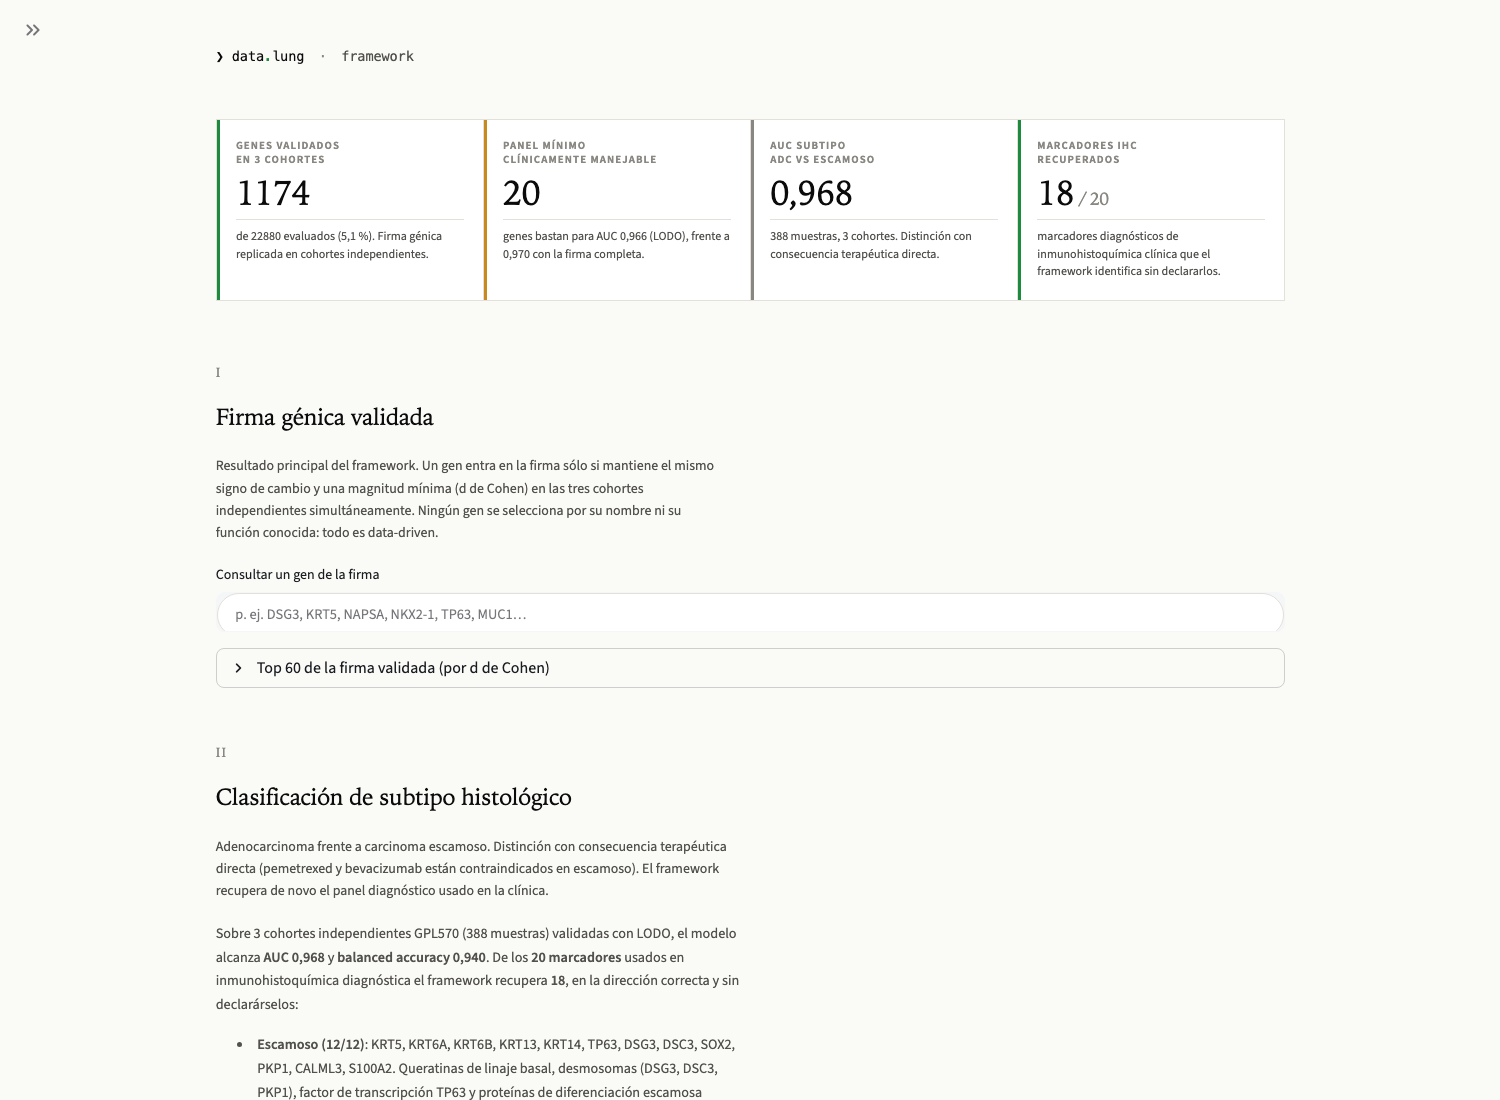
\includegraphics[width=0.9\linewidth]{figuras/interfaz/06_resultados.png}
  \caption{Capítulo \emph{Resultados}. Se aprecia la cabecera de cuatro
  tarjetas, el buscador de gen y el inicio de la sección de subtipo.}
  \label{fig:if_res}
\end{figure}

\section*{Vista 7: Cohortes individuales}
\addcontentsline{toc}{section}{Vista 7: Cohortes individuales}

El capítulo \emph{Cohortes} (figura~\ref{fig:if_cohortes}) proporciona
un \emph{drill-down} por cohorte: un desplegable permite elegir un
GSE\dots\ concreto y la interfaz muestra, para esa cohorte:

\begin{itemize}
  \item Tres cifras: número de muestras (con desglose sanas/enfermas),
  número de genes diferencialmente expresados a $\mathrm{FDR}<0{,}05$ y
  $<0{,}01$, y AUC máximo del ML local.
  \item Tabla de rendimiento por modelo (LR-L1, RF, SVM) sobre la
  cohorte, con validación interna.
  \item Tabla \emph{top 30} de genes diferencialmente expresados
  (ordenados por p-valor ajustado, con logFC y $p$-value en notación
  científica).
  \item Tabla \emph{top 20} de genes por peso en el ML local.
  \item Tres figuras exploratorias (PCA, volcano plot y heatmap) con
  título y descripción breve, siguiendo el mismo formato que las figuras
  globales del capítulo Resultados.
  \item Un desplegable con el informe biológico narrativo generado por
  el pipeline (\texttt{informe\_biologico.txt}) para esa cohorte.
\end{itemize}

Esta vista sirve como capa de auditoría por cohorte: complementa a la
media LODO de la cabecera principal permitiendo comprobar si algún
resultado agregado está impulsado por una cohorte en particular.

\begin{figure}[H]
  \centering
  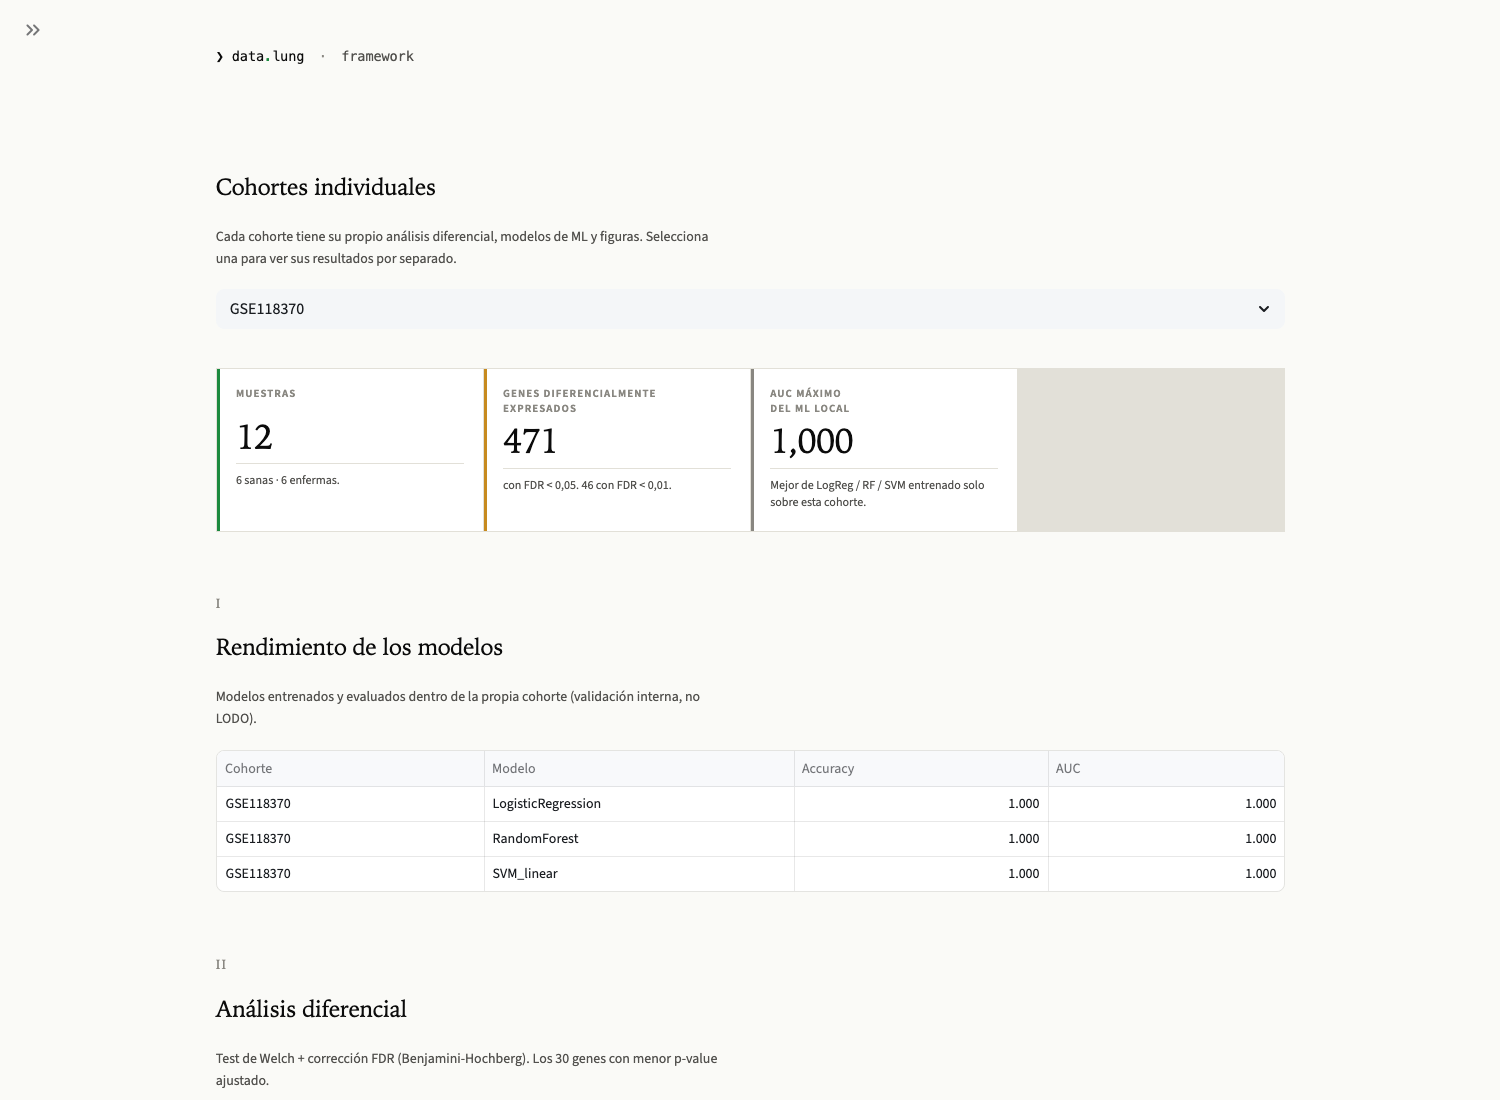
\includegraphics[width=0.9\linewidth]{figuras/interfaz/07_cohortes.png}
  \caption{Capítulo \emph{Cohortes}. Selector de cohorte y bloque de
  cifras por dataset.}
  \label{fig:if_cohortes}
\end{figure}

\section*{Vista 8: Conclusiones}
\addcontentsline{toc}{section}{Vista 8: Conclusiones}

El capítulo \emph{Conclusiones} (figura~\ref{fig:if_conclusiones})
reproduce el texto de las conclusiones del trabajo, organizado en cuatro
secciones: biomarcadores identificados, resultados de rendimiento,
aplicaciones clínicas y de investigación, y alcance del modelo con
trabajo futuro. Las listas de biomarcadores y las cifras de rendimiento
se leen dinámicamente del JSON y de los CSV, lo que garantiza la
coherencia entre el capítulo visual y los resultados subyacentes.

\begin{figure}[H]
  \centering
  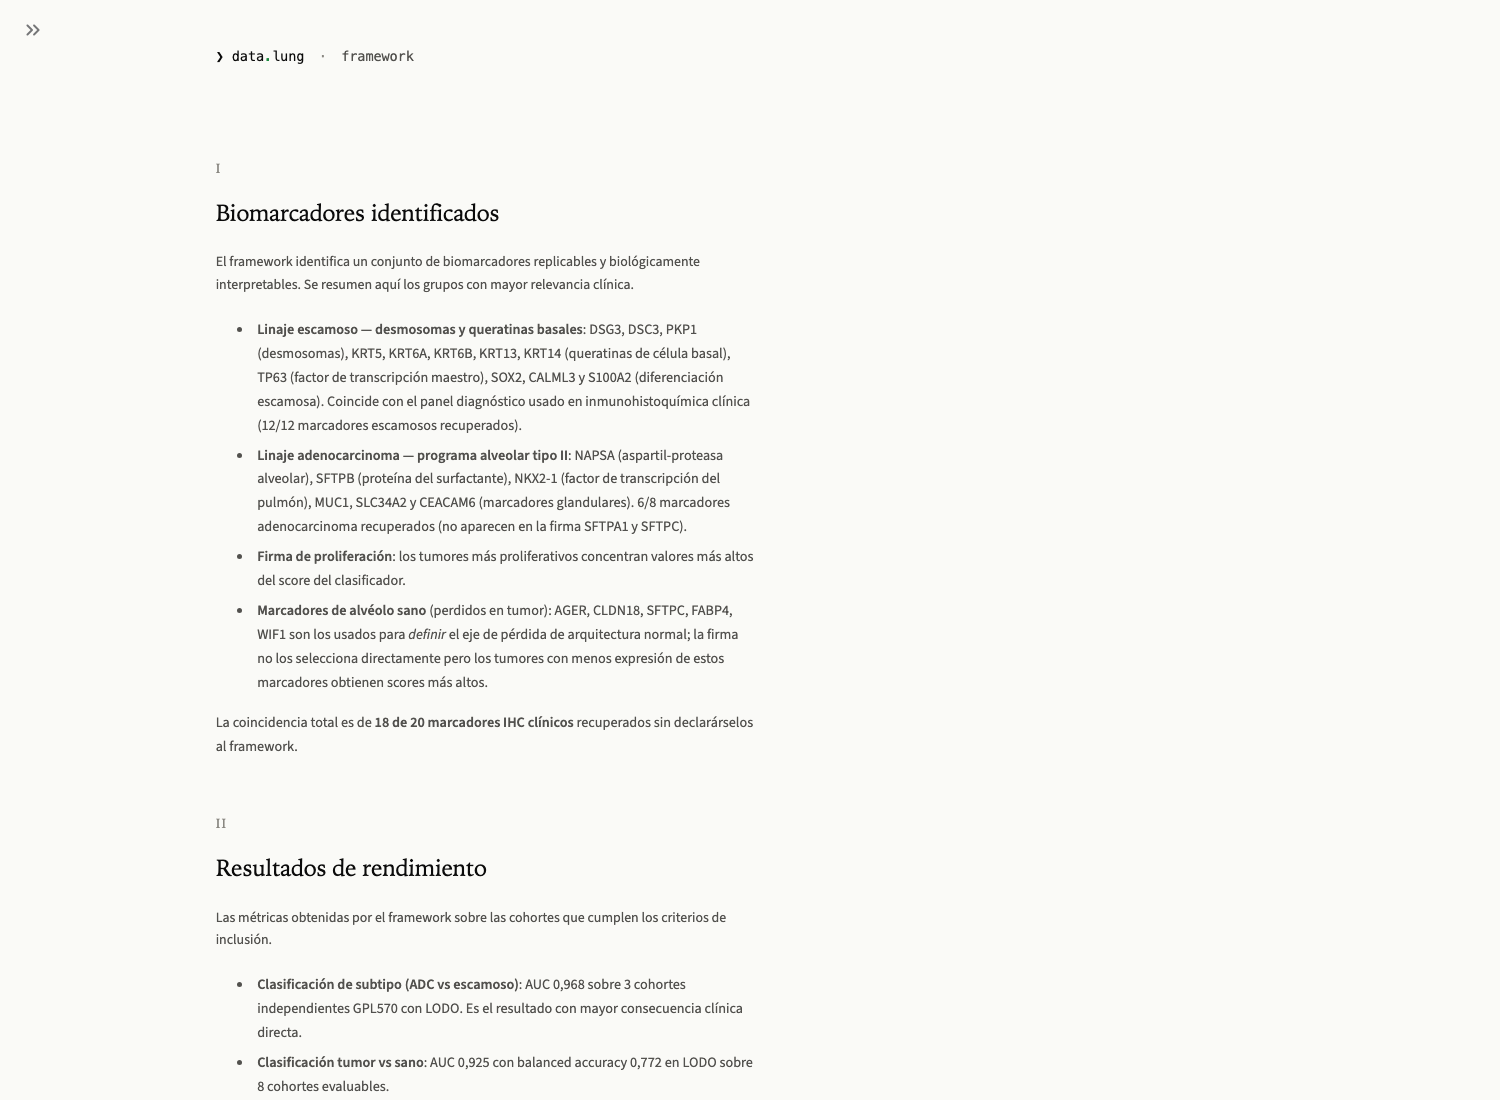
\includegraphics[width=0.9\linewidth]{figuras/interfaz/08_conclusiones.png}
  \caption{Capítulo \emph{Conclusiones}. Lista de biomarcadores por
  linaje con cifras de recuperación IHC.}
  \label{fig:if_conclusiones}
\end{figure}

\section*{Detalles técnicos y patrones de diseño}
\addcontentsline{toc}{section}{Detalles técnicos y patrones de diseño}

Algunos detalles técnicos relevantes de la implementación:

\begin{description}
  \item[Cifras nunca hardcodeadas.] Toda cifra visible en la interfaz se
  obtiene de \texttt{paso12\_datos.py} y en última instancia de un
  CSV/JSON. Cuando se detectó que \texttt{auc\_firma\_completa} del JSON
  guardaba por error el máximo de la curva del panel en lugar de la AUC
  con la firma completa, la función \texttt{resumen\_firma()} pasó a
  sobrescribir ese campo leyendo el valor correcto de
  \texttt{PANEL\_MINIMO\_CURVA.csv}, sin necesidad de regenerar el JSON.

  \item[Animación de conteo.] Las cifras del hero se animan con
  \emph{count-up} y \emph{easing} cúbico. El script se inyecta con
  \texttt{st.components.v1.html(height=0)} y usa el \emph{scheduler}
  del \texttt{window.parent} porque el navegador pausa
  \texttt{requestAnimationFrame} en iframes de altura cero, lo que
  provocaba que los contadores se congelaran en cero.

  \item[Estilo consistente con paleta verde terminal.] Los colores del
  dashboard (verde \texttt{\#1c8a3f} de acento, gris \texttt{\#fafaf7}
  de plano, tipografía serif y sans coordinadas) se definen en la
  cabecera CSS del dashboard y se aplican tanto a las tarjetas como a
  las burbujas del chat, al buscador de gen y a los bloques
  interpretativos de las figuras.

  \item[Navegación por capítulos vía \texttt{session\_state}.] En lugar
  de \texttt{st.tabs}, cada capítulo se muestra solo (según
  \texttt{st.session\_state.capitulo}) y se cambia mediante botones del
  \emph{sidebar}. Esto evita que el usuario vea contenidos irrelevantes
  al capítulo activo y permite una URL limpia.

  \item[Test de coherencia.] La suite \texttt{tests/test\_alineamiento.py}
  incluye un test que carga todas las cohortes disponibles y comprueba
  que muestra y etiqueta están alineadas por \texttt{geo\_accession}.
  Cuando no hay datos locales (por ejemplo en el runner de CI), el test
  se salta con \texttt{pytest.skip}.
\end{description}
